\documentclass{article}[12pt]
\usepackage{color}
\usepackage[normalem]{ulem}
\usepackage{times}
\usepackage{listings}
\usepackage{fullpage}
\usepackage{amsmath}
\usepackage{amssymb}
\usepackage{tikz}
\def \R {\mathbb R}
\def \imp {\Longrightarrow}
\def \eps {\varepsilon}
\def \Inf {{\sf Inf}}
\newenvironment{proof}{{\bf Proof.  }}{\hfill$\Box$}
\newtheorem{theorem}{Theorem}[section]
\newtheorem{definition}{Definition}[section]
\newtheorem{corollary}{Corollary}[section]
\newtheorem{lemma}{Lemma}[section]
\newtheorem{claim}{Claim}[section]
\setlength {\parskip}{2pt}
\setlength{\parindent}{0pt}

\newcommand{\headings}[4]{\noindent {\bf Assignment 6 CME241} \hfill {{\bf Author:} Nicolas Sanchez} \\
{} \hfill {{\bf Due Date:} #2} \\

\rule[0.1in]{\textwidth}{0.025in}
}

\newcommand{\klnote}[1]{{\color{red} #1}}
\newcommand{\klsout}[1]{{\color{red} \sout{#1}}}

\begin{document}

\headings{\#1}{Tuesday, October 8, 10:30am}\section{} 



\section{Implementation from scratch of MC and TD}
We implement the algorithms from scratch as shown below and in mc\_scratch.py

\begin{lstlisting}
def mc_prediction_tabular(
        traces: Iterable[Iterable[mp.TransitionStep[S]]],
        gamma: float,
        iters_max: int,
        l_rate: float = 0.1,
        tolerance: float = 1e-6
) -> Dict[S,float]:
    episodes = (returns(trace, gamma, tolerance) for trace in traces)
    iter_count = 0

    count_dict = {}
    sum_dict = {}

    for episode in episodes:
        iter_count +=1
        for step in episode:
            count_dict[step.state] = count_dict.get(step.state, 0) + 1
            sum_dict[step.state] = sum_dict.get(step.state, 0.0) + \
                    (step.return_ - sum_dict.get(step.state, 0.0))*(1./iter_count)
        if iter_count > iters_max:
            break
    MC_approx = {}
    for s in sum_dict:
        MC_approx[s] = sum_dict[s]/float(count_dict[s])

    return MC_approx

def td_prediction_tabular(
        transitions: Iterable[mp.TransitionStep[S]],
        alpha_fn: Callable[[int], float],
        gamma: float,
        iters_max :int
) -> Dict[S,float]:

    iter_count = 0
    counts = {}
    vals = {}

    for tr_step in transitions:
        iter_count +=1
        est_val = tr_step.reward + gamma*vals.get(tr_step.next_state, 0)
        counts[tr_step.state] = counts.get(tr_step.state, 0) + 1
        weight: float = alpha_fn(counts.get(tr_step.state, 0))
        vals[tr_step.state] = weight * est_val + (1 - weight) * vals.get(tr_step.state, 0.)
        if iter_count > iters_max:
            break

    return vals
   
\end{lstlisting}
We run the above for the case of the Simple Inventory problem and obtain very similar value functions, suggesting correct implementation. Here MC approx and TD approx were the functions provided in class whereas the tabular versions were the ones created using the above from-scratch implementations:
\begin{figure}[h!]
  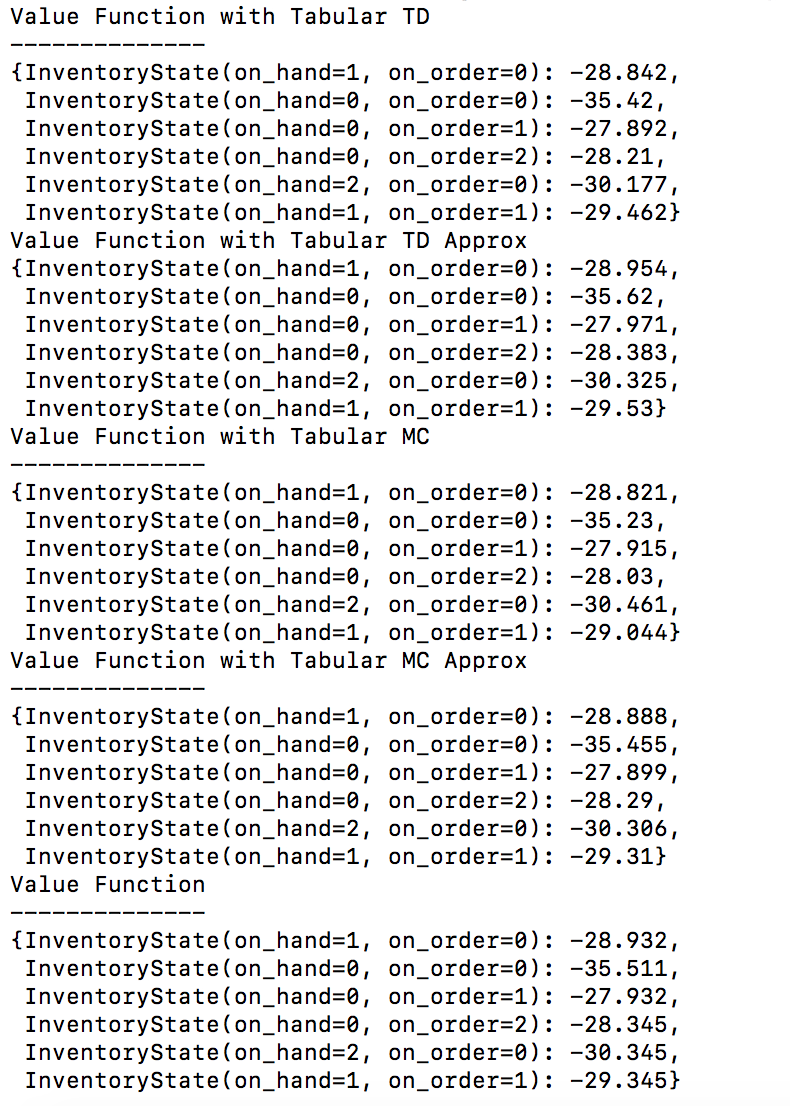
\includegraphics[width=0.5\linewidth]{scratch_values.png}
  \caption{Similar Values for all prediction models}
  \label{fig:optPol1}
\end{figure}


\section{Implementation Random Walk in 2D}

We implement the random walk in 2D in random\_walk\_mrp.py. The most important function is simply the get\_transition\_map.py which we include here:

\begin{lstlisting}
    def get_transition_map(self) -> \
            Mapping[Tuple[int,int], Optional[Categorical[Tuple[Tuple[int,int], float]]]]:


        d: Dict[Tuple[int,int], Optional[Categorical[Tuple[Tuple[int,int], float]]]] = {
            (i,j): Categorical({
                ((i + 1,j), 0. if i < self.barrier_right - 1 else 1.): self.p_right,
                ((i,j+1), 0. if j < self.barrier_top - 1 else 1.): self.p_up,
                ((i - 1,j), 0.): self.p_left,
                ((i,j-1), 0.): self.p_down
            }) for i in range(1, self.barrier_right) for j in range(1,self.barrier_top)
        }
        for i in range(self.barrier_right):
            d[(i,0)] = None
            d[(i,self.barrier_top)] = None

        for j in range(self.barrier_right):
            d[(0,j)] = None
            d[(self.barrier_right,j)] = None

        return d
\end{lstlisting}

When comparing the convergence results for MC and TD we arrive at similar conclusions as we did in class. The convergence graph is given here.
\begin{figure}[h]
  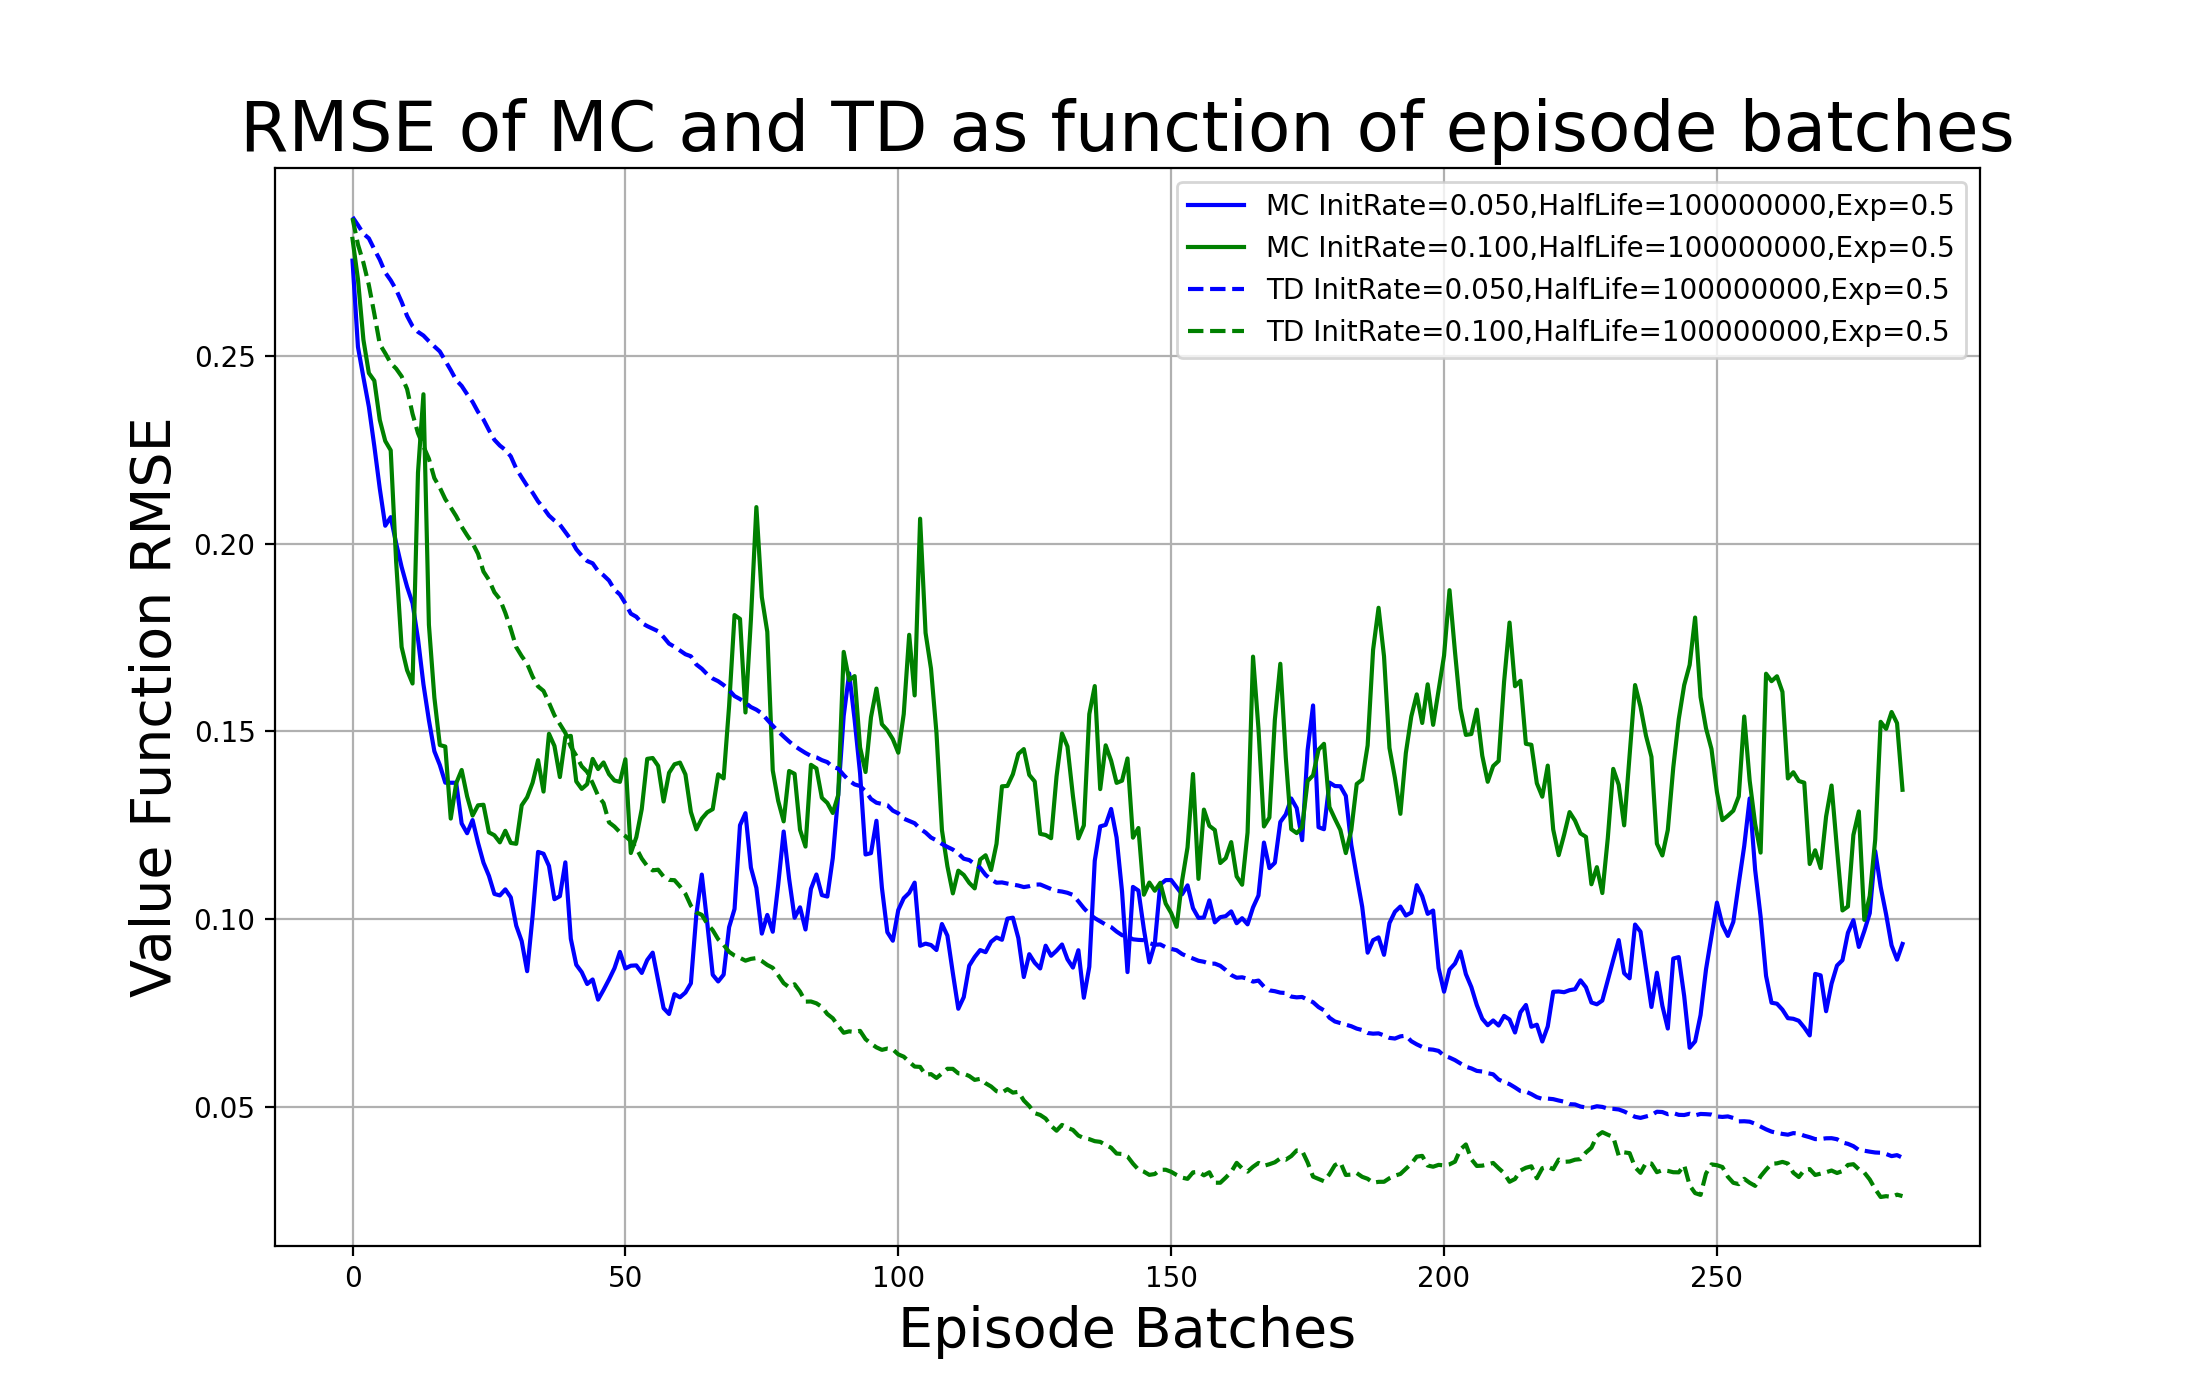
\includegraphics[width=\linewidth]{conv_graph.png}
  \caption{Convergence speeds for TD and MC on RandomWalk2D}
  \label{fig:optPol1}
\end{figure}

We note that the more complex problem with likely longer episode duration means that we required more episodes and higher learning rates compared to the 1D case. However, accounting for that higher complexity we arrive at similar conclusions. MC seems to come closer to the final value quicker initially - intuitively this makes sense as the TD is highly bias initially when initiated to 0 on all states. MC is more agnostic to initial state. However TD overtime provides a more robust (better and less variance) convergence to true value function independent of the learning rate. 

\end{document}
